\subsection{Qualitative1: Distribution and Regression Analysis}

As a baseline for the subsequent, more complex qualitative profiling, we first performed a focused set of distribution and regression tests centered on two questions: (1) whether measured text-derived sentiment and individualism--collectivism (IC) orientation differ between WEIRD and non-WEIRD populations when all participants are included, and (2) whether analytical-minus-emotional trust change can be predicted from sentiment and collectivity scores with group-specific trends.

As in the prior qualitative analyses, participant-level sentiment was computed as the mean VADER compound score across available free-text fields (AI Interaction Feeling, Need Model Understanding, Job Screening Feeling, Explanation Comment). Participant-level collectivity was computed from the IC lexical contrast score (collectivist minus individualistic language signal) aggregated across the same text fields. Trust-change outcomes were normalized pre--post z-score changes, and for regression we used the derived dependent variable analytical-minus-emotional change ($\Delta_{A-E} = z_{analytical} - z_{emotional}$).

\textbf{Analysis 1: Sentiment distribution by WEIRD/non-WEIRD (all participants).} The left panel of Figure~\ref{fig:qualitative1} shows boxplots (with whiskers and participant-level points) for participant mean sentiment, grouped only by WEIRD and non-WEIRD status. A Welch test found no significant difference between WEIRD and non-WEIRD sentiment distributions ($p=.883$; $n_{WEIRD}=157$, $n_{non-WEIRD}=347$). As a reference check, the aggregate negative-vs-positive split across all participants was strongly separated by construction ($p<.001$).

\textbf{Analysis 2: IC distribution by WEIRD/non-WEIRD (all participants).} The second panel shows boxplots for participant IC scores (collectivist minus individualistic language signal), again grouped only by WEIRD and non-WEIRD status. The WEIRD vs non-WEIRD difference was not significant ($p=.332$; $n_{WEIRD}=157$, $n_{non-WEIRD}=347$). As a reference check, the aggregate individualistic-vs-collectivist split across all participants was strongly separated ($p<.001$).

\textbf{Analysis 3: Group-split regression of analytical-minus-emotional trust change.} The right two panels report regressions predicting $\Delta_{A-E}$ from sentiment and collectivity with separate WEIRD and non-WEIRD trend lines. Dots represent binned mean values over nearby predictor ranges, with whiskers showing within-bin standard deviations. For sentiment, both group-specific slopes were positive and significant (WEIRD: $\beta=1.265$, $p=.015$, $R^2=.038$; non-WEIRD: $\beta=1.324$, $p<.001$, $R^2=.047$), indicating that more positive language was associated with relatively larger analytical-vs-emotional trust change in both populations. For collectivity, slopes were negative but non-significant in both groups (WEIRD: $\beta=-0.324$, $p=.309$, $R^2=.007$; non-WEIRD: $\beta=-0.122$, $p=.554$, $R^2=.001$), indicating limited linear predictive value of IC score alone for this contrast outcome.

Taken together, these baseline results show that simple group-level distribution shifts in sentiment and IC are weak, but sentiment retains a robust group-consistent linear association with analytical-minus-emotional trust change, whereas collectivity does not show a comparable linear signal.

\begin{figure}[htbp]
\centering
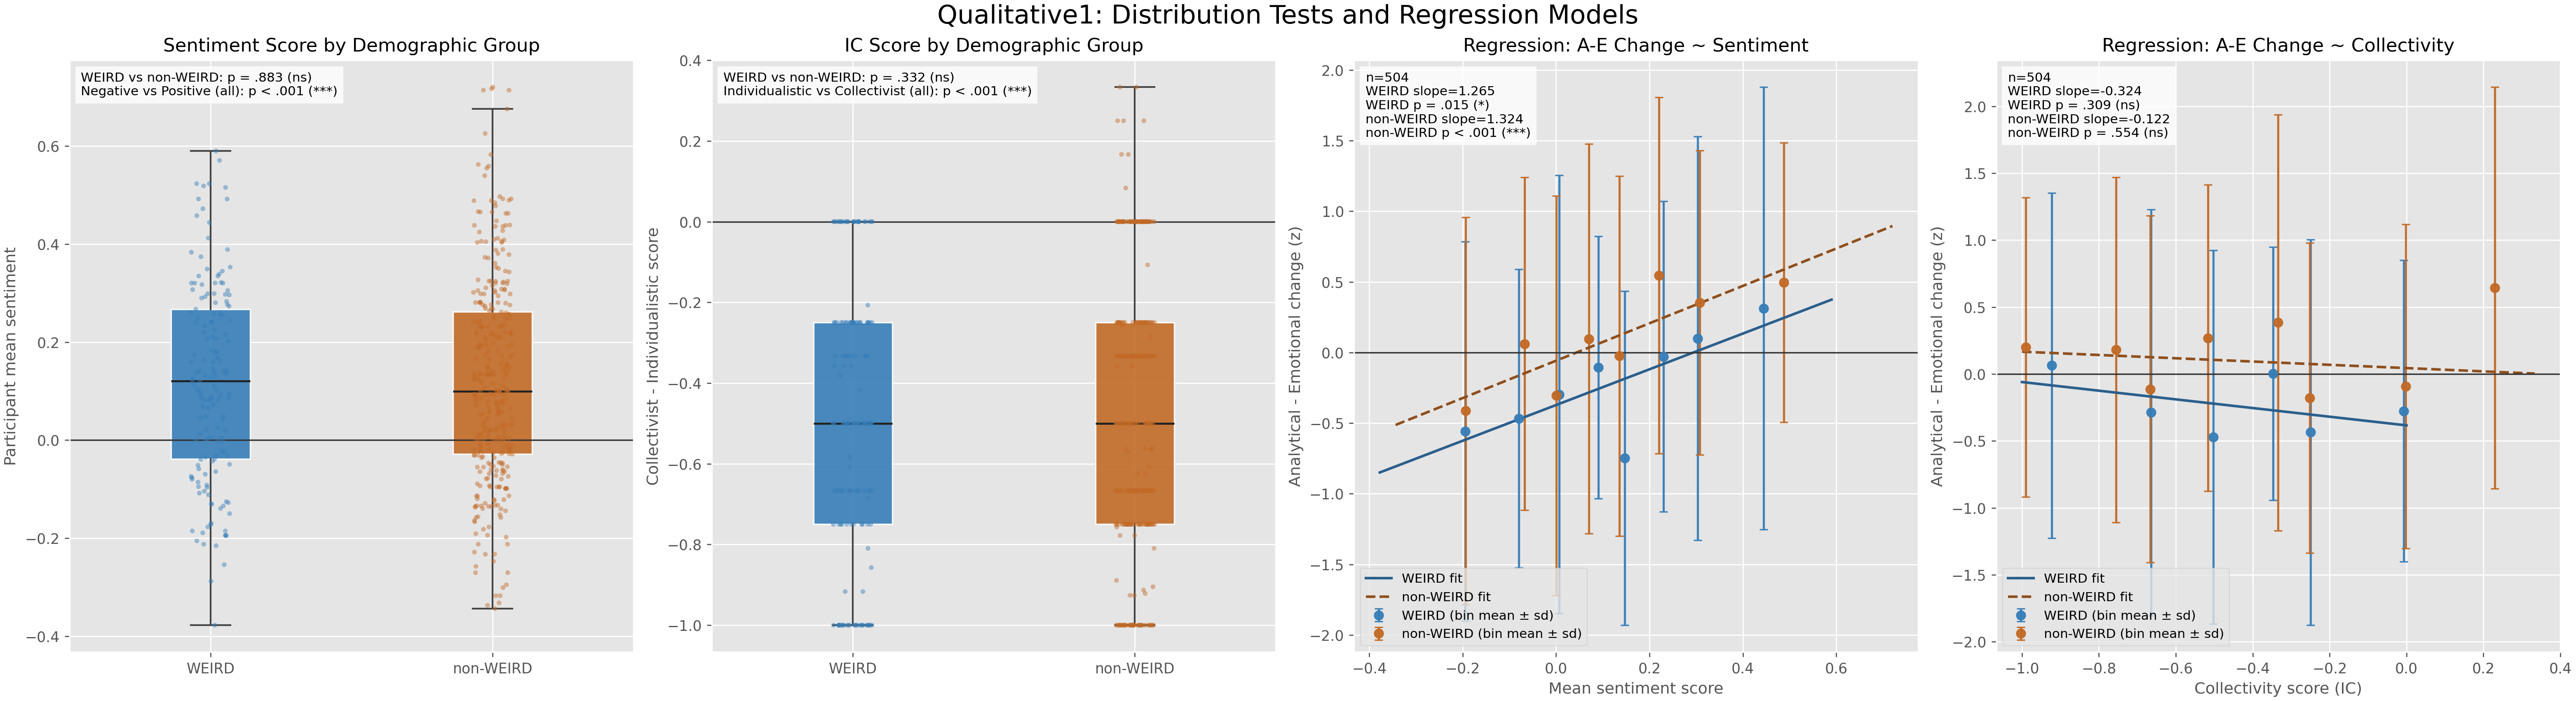
\includegraphics[width=0.99\linewidth]{Figures/qualitative1.png}
\caption{Qualitative1 analysis: (left) sentiment score distributions by polarity and demographic group, (middle-left) IC score distributions by orientation and demographic group, (middle-right) regression of analytical-minus-emotional trust change on sentiment score, and (right) regression of analytical-minus-emotional trust change on collectivity score. Boxplots include whiskers and participant-level dots; regression panels include fitted lines and significance summaries.}
\label{fig:qualitative1}
\end{figure}
